\frontmatter

{\pagestyle{empty} % Blocca le pagine dal venire considerate nella numerazione

{
	\centering
	
	~
	
	\vspace{24pt}
	{\scshape\Huge Il gioco\\di Ender \par}
}

\cleardoublepage

\newlength\drop
\makeatletter
\newcommand*\titleM{\begingroup% Misericords, T&H p 153
	\setlength\drop{0.08\textheight}
	\centering
	\vspace*{\drop}
	{\Huge\bfseries Il gioco di Ender}\\[\baselineskip]
	{\scshape Orson Scott Card}\\[\baselineskip]
	\vfill
	{\large\scshape \phantom{the author}}\par
	\vfill
	{\large\scshape DiracEdizioni \img{Immagini/DiracEdizioniLogo.png}}\par
	\endgroup}
\makeatother
	
\titleM

\newpage\blankpage

\space\pagebreak

\null\vfill % Portiamo il testo del copy in basso

\begin{flushright}
	
		\footnotesize \textit{Il gioco di Ender}
		
		\bigskip
		
		COPYRIGHT © 2024 Orson Scott Card
		
		\bigskip
		
		Tutti i diritti riservati.\\
		Nessuna parte di questa pubblicazione può essere riprodotta,\\
		memorizzata o trasmessa in qualsiasi forma o con qualsiasi mezzo,\\
		elettronico, meccanico, di fotocopiatura, registrazione, scansione o altro\\
		senza il permesso scritto dell'editore. È illegale copiare questo libro, pubblicarlo\\ 
		su un sito web o distribuirlo con qualsiasi altro mezzo senza autorizzazione.
		
		\bigskip
		
		Questo romanzo è interamente un'opera di fantasia.\\
		I nomi, i personaggi e gli episodi in esso rappresentati\\
	    sono frutto dell'immaginazione dell'autore.\\
	    Qualsiasi somiglianza con persone reali, vive o morte, eventi o località\\
	    è del tutto casuale.
		
		\bigskip
		
		\textonesuperior Edizione, 2024
		
		\bigskip
		
		\begin{tabular}{rl}
			ISBN--10:& 0-4847-9887-1\\ 
			ISBN--13:& 978-0-0203-7909-6\\ 
		\end{tabular}	
		
		\bigskip
		
		\begin{figure}[h]
			\begin{flushright}
				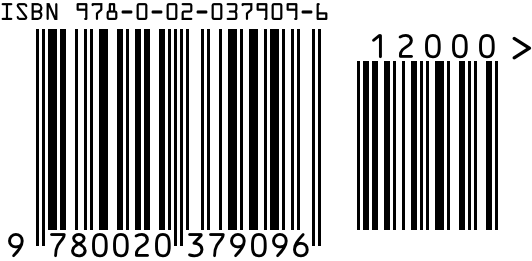
\includegraphics[width=0.3\linewidth]{Immagini/barcode_978-0-02-037909-6}
			\end{flushright}
		\end{figure}
		
		Pubblicato da DiracEdizioni \img{Immagini/DiracEdizioniLogo.png}
		
\end{flushright}
}
 
{\chapterstyle{bringhurst} \chapter*{PRESENTAZIONE}
	
\setcounter{page}{1}

\emph{{~}}

\emph{{~}}

\emph{{~}}

\emph{{Nato nello stato di Washington (negli Stati Uniti) e cresciuto in
		California e in Arizona, Orson Scott Card ha praticato vari mestieri
		prima di approdare alla carriera di scrittore di fantascienza. Ha
		iniziato infatti come direttore della Brigham Young University Press,
		una piccola casa editrice universitaria; è stato poi impresario di una
		compagnia teatrale (per cui ha composto anche delle opere), ed ha poi
		interrotto questa attività per recarsi in Brasile come missionario della
		chiesa dei mormoni. Tornato negli Stati Uniti ha lavorato presso vari
		editori dell'Utah. Infine, nel 1978 ha preso la decisione di dedicarsi
		completamente alla carriera di scrittore. Ora vive ad Orem, nello Utah,
		con la moglie Kristine Allen e il figlio Geoffrey, e, oltre a produrre
		narrativa fantascientifica, tiene anche un corso per scrittori
		all'università dello Utah a Salt Lake City.}}

\emph{{Card, che è certamente uno dei maggiori talenti fantascientifici
		tra gli scrittori delle ultime leve, ha iniziato la sua carriera proprio
		con la versione breve di questo «Il gioco di Ender», che apparve su
		«Analog» nel 1977 e lo aiutò a vincere il premio John W. Campbell jr.
		per il miglior autore esordiente dell'anno.}}

\emph{{In questi dieci anni di attività letteraria ha prodotto un certo
		numero di romanzi (sette, ci sembra) e molti racconti, alcuni dei quali
		sono stati raccolti in due antologie personali («Capitol» e
		«Unaccompanied Sonata»).}}

\emph{{Card, come molti altri tra gli autori delle ultime leve, non è
		partito come un vero fan della fantascienza, ma ci si è accostato solo
		poco per volta.}}{ «Scoprii la fantascienza nella mia prima avventura
	alla sezione adulta della biblioteca pubblica di Santa Clara, in
	California», \emph{dice lo stesso Card al riguardo.} «Avevo dieci o
	undici anni quando iniziai a leggere le antologie di Groff Conklin;
	``Cali me Joe'', di Poul Anderson; ``All You Zombies'', di Robert
	Heinlein, e decine di altre storie i cui titoli o autori ho dimenticato,
	che stimolarono la mia immaginazione. Ma abbandonai le letture
	fantascientifiche prima dei tredici anni e non ricominciai fino a quando
	un amico mi fece conoscere Bradbury (divorai ``I Sing the Body
	Electric'', e poi ``Dandelino Wine'' e qualsiasi altra cosa di suo su
	cui riuscissi a mettere mano). Mia cognata mi fece conoscere la trilogia
	della Fondazione e allora lessi tutti i libri di sf di Asimov che
	riuscii a trovare. Avevo circa vent'anni quando soccombetti alle
	pressioni sociali e lessi l'\,``Hobbit'', la cui lettura fu invero una
	sofferenza; ma poi lessi ``Il signore degli anelli'' e venni di colpo
	trasformato da lettore casuale, in un vero appassionato. Lessi Ellison,
	Le Guin e Clarke. Avevo letto in precedenza ``Tunnel in the Sky'' e
	``Citizen of the Galaxy'', ma quando arrivai a ``The Moon is a Harsh
	Mistress'' e ``Glory Road'', decisi che amavo davvero Heinlein. Soltanto
	di recente ho letto qualcosa di Niven, ma da allora mi sono bevuto tutti
	i suoi libri come un assetato a corto d'acqua. Non sono mai stato un fan
	che scriveva lettere in continuazione e non scoprii il fandom finché non
	vendetti la mia prima storia ad ``Analog''. Le mie letture tuttavia non
	sono mai state limitate solo alla sf: ho sempre letto con piacere libri
	di storia e biografie; e la letteratura per ragazzi mi piace in genere
	più della sf».}

\emph{{Come si vede dunque Card non è il tipico appassionato di sf che
		ha letto solo fantascienza fin da piccolo ed ha poi cominciato a
		scriverla non appena ha avuto l'età giusta. Le sue letture e i suoi
		interessi sono molto vari e ciò si riflette anche sulla qualità del suo
		stile.}}

\emph{{Fin dalle sue prime opere, come «Capitol» e «Hot Sleep», si può
		notare in lui una buona visione della trama, una notevole maturità, un
		realistico apprezzamento dei limiti degli esseri umani, e soprattutto
		una discreta tecnica letteraria. Card sa scrivere, e riesce in genere a
		trovare il giusto passo dell'azione, il giusto ritmo degli avvenimenti;
		nei suoi libri, e soprattutto in questo «Ender's Game» non ci sono punti
		deboli, non ci sono inutili lentezze, come nei migliori romanzi di
		Heinlein, cui questo romanzo è vagamente ispirato.}}

\emph{{Prima di giungere a questo «Ender's Game» Card ha composto altre
		opere di buona fattura, meritevoli anch'esse di essere conosciute dal
		nostro pubblico, come «A Planet Called Treason», «Songmaster» e «Hart's
		Hope», un'ottima fantasy che si distacca dai canoni dell'epica eroica
		moderna alla Howard, per riagganciarsi invece alle tradizioni antiche
		delle fiabe e delle leggende in un continuo gioco di emozioni e
		filosofie, di politica e di magia che lo rendono davvero memorabile.}}

\emph{{Con «Il gioco di Ender» invece Card è riuscito a dare nuovo
		vigore e nuovo fascino a un genere fantascientifico che sembrava ormai
		destinato a divenire un puro cliché: l'allenamento di un cadetto
		spaziale destinato a prender parte a una guerra contro nemici di forma
		insettoide. Dickson con il suo «Generale genetico» e Heinlein con tutta
		una serie di ottimi «juveniles» (a partire da «Cittadino della galassia»
		e da « Tunnel in the Sky» fino a «Space Cadet» e «Starman Jones»)
		avevano ormai codificato e canonizzato questo tipo di avventura spaziale
		portandolo a un livello di perfezione forse insuperabile.}}

\emph{{E invece ecco arrivare Orson Scott Card e produrre così, di
		getto, una storia nuova, interessante, avvincente, incentrata su un
		bambino, «Ender» Wiggins, che ha le doti di un superbo comandante e
		viene forzato ad una precoce maturità attraverso un interminabile e
		ossessionante addestramento basato sui «giochi dì guerra».}}

\emph{{Ciò che rende questo libro così speciale, tanto da portarlo a una
		facile e indiscussa vittoria sugli altri concorrenti all'Hugo e al
		Nebula del 1986, è l'umanità che lo pervade, la profonda compassione che
		trapela per Ender e i suoi sfortunati compagni. I bambini non sono
		soltanto degli strumenti da utilizzare per scopi e necessità militari,
		sembra voler affermare Card, mentre sottolinea e descrive la grande
		differenza di educazione tra Ender e i suoi compagni, costretti a
		continui addestramenti, a continui combattimenti (anche se solo
		simulati) in uno stato di estrema tensione nervosa, e gli altri bambini
		della sua età, che giocano felici e sereni nei giardini della Terra,
		inconsapevoli della minaccia aliena e soprattutto liberi dal fardello
		psicologico di dover affrontare tale minaccia con la responsabilità del
		destino dell'intera razza umana sulle spalle.}}

\emph{{E anche gli addestratori, che pure costringono bambini di otto o
		nove anni a una vita di sforzi e tensioni incredibili, non sono mai
		visti da Card come esseri disumani, inflessibili sergenti di ferro da
		film di guerra. Al contrario, gli adulti di questo romanzo sono figure
		altrettanto ben delineate. Umani al punto di osservare la propria
		crudeltà con un qualcosa di molto simile alla disperazione di chi non ha
		altra scelta e deve eseguire un compito ingrato e difficile, come quello
		di fare di Ender un bambino-generale che da una parte abbia un `abilità
		spietata e dall'altra conservi, in un'apparente contraddizione, la sua
		«umanità».}}

\emph{{In sostanza, un libro che contiene molto più di quello che
		potrebbe apparire a prima vista e che è molto di più di una semplice
		avventura spaziale: non che la storia non sia}}{ anche \emph{un'ottima e
		avvincente avventura, ma la profonda e memorabile umanità dei personaggi
		la portano a trascendere i confini del puro sottogenere fino a
		raggiungere lo status di classico della fantascienza.}}

{~}

{Sandro Pergameno}

}

